\UseRawInputEncoding

%%%%%%%%%%%%%%%%%%%%%%%%%%%%%%%%%%%%%%%%%%%%%%%%%%%%%%%%%%%%%%%%%%%%%%%%%%%%%%%%
%% Settings
%%%%%%%%%%%%%%%%%%%%%%%%%%%%%%%%%%%%%%%%%%%%%%%%%%%%%%%%%%%%%%%%%%%%%%%%%%%%%%%%
%% Columns
\documentclass[final,3p,times,twocolumn]{elsarticle}
%% Use the options 1p,twocolumn; 3p; 3p,twocolumn; 5p; or 5p,twocolumn
%% for a journal layout:
%% \documentclass[final,1p,times]{elsarticle}
%% \documentclass[final,1p,times,twocolumn]{elsarticle}
%% \documentclass[final,3p,times]{elsarticle}
%% \documentclass[final,3p,times,twocolumn]{elsarticle}
%% \documentclass[final,5p,times]{elsarticle}
%% \documentclass[final,5p,times,twocolumn]{elsarticle}
%% \documentclass[preprint,review,12pt]{elsarticle}

%% Image width
\newlength{\imagewidth}
\newlength{\imagescale}
%% preamble
\usepackage[english]{babel}
\usepackage[table]{xcolor} % For coloring tables
\usepackage{booktabs} % For professional quality tables
\usepackage{colortbl} % For coloring cells in tables
\usepackage{amsmath, amssymb} % For mathematical symbols and environments
\usepackage{amsthm} % For theorem-like environments
\usepackage{lipsum} % just for sample text
\usepackage{natbib}
\usepackage{graphicx}
\usepackage{indentfirst}
\usepackage{bashful}
\usepackage[margin=10pt,font=small,labelfont=bf,labelsep=endash]{caption}
\usepackage{graphicx}
\usepackage{calc}
\usepackage[T1]{fontenc} % [REVISED]
\usepackage[utf8]{inputenc} % [REVISED]
\usepackage{hyperref}
\usepackage{accsupp}
%% Line numbers
\linespread{1.1}
% \linenumbers
% Tables
\usepackage[pass]{geometry}
\usepackage{pdflscape}
\usepackage{csvsimple}
\usepackage{xltabular}
\usepackage{booktabs}
\usepackage{siunitx}
\usepackage{makecell}
\sisetup{round-mode=figures,round-precision=3}
\renewcommand\theadfont{\bfseries}
\renewcommand\theadalign{c}
\newcolumntype{C}[1]{>{\centering\arraybackslash}m{#1}}
\renewcommand{\arraystretch}{1.5}
\definecolor{lightgray}{gray}{0.95}

%% Diff
\usepackage{xcolor}
% Define commands for highlighting
% diff
\usepackage[most]{tcolorbox} % for boxes with transparency
% Define colors with transparency (opacity value)
\definecolor{GreenBG}{rgb}{0,1,0}
\definecolor{RedBG}{rgb}{1,0,0}
% Define tcolorbox environments for highlighting
\newtcbox{\greenhighlight}[1][]{%
  on line,
  colframe=GreenBG,
  colback=GreenBG!50!white, % 50% transparent green
  boxrule=0pt,
  arc=0pt,
  boxsep=0pt,
  left=1pt,
  right=1pt,
  top=2pt,
  bottom=2pt,
  tcbox raise base
}
\newtcbox{\redhighlight}[1][]{%
  on line,
  colframe=RedBG,
  colback=RedBG!50!white, % 50% transparent red
  boxrule=0pt,
  arc=0pt,
  boxsep=0pt,
  left=1pt,
  right=1pt,
  top=2pt,
  bottom=2pt,
  tcbox raise base
}
\newcommand{\REDSTARTS}{\color{red}}
\newcommand{\REDENDS}{\color{black}}
\newcommand{\GREENSTARTS}{\color{green}}
\newcommand{\GREENENDS}{\color{black}}
%%%%%%%%%%%%%%%%%%%%%%%%%%%%%%%%%%%%%%%%%%%%%%%%%%%%%%%%%%%%%%%%%%%%%%%%%%%%%%%%
%% Journal Name
%%%%%%%%%%%%%%%%%%%%%%%%%%%%%%%%%%%%%%%%%%%%%%%%%%%%%%%%%%%%%%%%%%%%%%%%%%%%%%%%
\journal{Heliyon}
%%%%%%%%%%%%%%%%%%%%%%%%%%%%%%%%%%%%%%%%%%%%%%%%%%%%%%%%%%%%%%%%%%%%%%%%%%%%%%%%
%% Document Starts
%%%%%%%%%%%%%%%%%%%%%%%%%%%%%%%%%%%%%%%%%%%%%%%%%%%%%%%%%%%%%%%%%%%%%%%%%%%%%%%%
\begin{document}


%%%%%%%%%%%%%%%%%%%%%%%%%%%%%%%%%%%%%%%%%%%%%%%%%%%%%%%%%%%%%%%%%%%%%%%%%%%%%%%%
%% Frontmatter
%%%%%%%%%%%%%%%%%%%%%%%%%%%%%%%%%%%%%%%%%%%%%%%%%%%%%%%%%%%%%%%%%%%%%%%%%%%%%%%%
\begin{frontmatter}
\begin{highlights}
\pdfbookmark[1]{Highlights}{highlights}

\item Neural trajectories in the hippocampus exhibited greater variability during a working memory (WM) task compared to those in the entorhinal cortex and amygdala regions.

\item The distance of neural trajectories between encoding and retrieval states in the hippocampus was memory-load dependent during a WM task.


\item Hippocampal neural trajectories fluctuated between the encoding and retrieval states in a task-dependent manner during both baseline and sharp-wave ripple (SWR) periods.

\item Hippocampal neural trajectories shifted from encoding to retrieval states during SWR period.

\end{highlights}\title{
Hippocampal neural fluctuations between memory encoding and retrieval states during a working memory task in humans
}\author[1]{Yusuke Watanabe\corref{cor1}}
\author[2,3,4]{Yuji Ikegaya}
\author[1,5]{Takufumi Yanagisawa}

\address[1]{Institute for Advanced Cocreation studies, Osaka University, 2-2 Yamadaoka, Suita, 565-0871, Osaka, Japan}
\address[2]{Graduate School of Pharmaceutical Sciences, The University of Tokyo, 7-3-1 Hongo, Tokyo, 113-0033, Japan}
\address[3]{Institute for AI and Beyond, The University of Tokyo, 7-3-1 Hongo, Tokyo, 113-0033, Japan}
\address[4]{Center for Information and Neural Networks, National Institute of Information and Communications Technology, 1-4 Yamadaoka, Suita City, 565-0871, Osaka, Japan}
\address[5]{Department of Neurosurgery, Osaka University Graduate School of Medicine, 2-2 Yamadaoka, Osaka, 565-0871, Japan}

\cortext[cor1]{Corresponding author. Tel: +81-6-6879-3652}%%Graphical abstract
%\pdfbookmark[1]{Graphical Abstract}{graphicalabstract}        
%\begin{graphicalabstract}
%\includegraphics{grabs}
%\end{graphicalabstract}
\begin{abstract}
\pdfbookmark[1]{Abstract}{abstract}
Working memory (WM) plays a critical role in diverse cognitive functions, yet its neural mechanisms remain largely unelucidated. An emerging area of focus is the role of the hippocampus and sharp wave-ripple complexes (SWRs) – fleeting, synchronized neural events in the hippocampus – in memory consolidation and retrieval, although their connection to WM tasks remains unclear. Recent research suggests that multiunit activity patterns in the hippocampus may function concurrently with SWRs, displaying unique dynamics during WM tasks. We conducted an analysis of an electroencephalogram dataset from the medial temporal lobe (MTL) in nine epilepsy patients during an eight-second Sternberg task. Low-dimensional neural representations, or 'trajectories', within the MTL were isolated using Gaussian-process factor analysis while performing the WM task. The results reveal significant differences in the neural trajectories in the hippocampus in comparison to the entorhinal cortex and the amygdala. Furthermore, the variance in trajectories between the encoding and retrieval phases seems to be memory load-dependent. Interestingly, hippocampal trajectories vary during the retrieval phase, indicating task-dependent shifts between encoding and retrieval states which occur during both baseline and SWR events. These shifts from encoding to retrieval states are synchronized with the occurrence of SWRs, emphasizing the crucial role of the hippocampus in WM tasks. This suggests a new hypothesis: the hippocampus changes its functional state from encoding to retrieval during the presence of SWRs.
\end{abstract}% \pdfbookmark[1]{Keywords}{keywords}                
\begin{keyword}
working memory \sep WM \sep memory load \sep hippocampus \sep sharp-wave ripples \sep SWR \sep humans
\end{keyword}
\end{frontmatter}

%%%%%%%%%%%%%%%%%%%%%%%%%%%%%%%%%%%%%%%%%%%%%%%%%%%%%%%%%%%%%%%%%%%%%%%%%%%%%%%%
%% IMRaD
%%%%%%%%%%%%%%%%%%%%%%%%%%%%%%%%%%%%%%%%%%%%%%%%%%%%%%%%%%%%%%%%%%%%%%%%%%%%%%%%
\section{Introduction}
Working memory (WM) is essential for various daily tasks, yet we still lack full comprehension of the associated neural mechanisms. In particular, the hippocampus, a crucial region for memory in the brain, demands continued investigation \cite{scoville_loss_1957,squire_legacy_2009,boran_persistent_2019,kaminski_persistently_2017,kornblith_persistent_2017,faraut_dataset_2018,borders_hippocampus_2022,li_functional_2023,dimakopoulos_information_2022}. Improving our understanding of the hippocampus's role in working memory could provide enhanced insights into cognitive processes and stimulate the advancement of cognitive training strategies and interventions. 

\indent
Hippocampally-generated sharp wave ripples (SWR), which are transient and synchronous oscillations, are linked to fundamental cognitive functions such as memory replay \cite{wilson_reactivation_1994,nadasdy_replay_1999,lee_memory_2002,davidson_hippocampal_2009}, memory consolidation \cite{girardeau_selective_2009,ego-stengel_disruption_2010,fernandez-ruiz_long-duration_2019,kim_corticalhippocampal_2022}, memory recall \cite{wu_hippocampal_2017,norman_hippocampal_2019,norman_hippocampal_2021}, and neural plasticity \cite{behrens_induction_2005,norimoto_hippocampal_2018}. Therefore, SWRs may play a key role in hippocampal processing and potentially influence working memory performance. Nonetheless, research investigating the impact of SWRs on working memory is limited \cite{jadhav_awake_2012}, mainly focusing on rodent models performing navigation tasks without clearly differentiating between specific timings of memory recall and acquisition.

\indent
Furthermore, it has been observed that hippocampal neurons exhibit low-dimensional representations during WM tasks. Notably, the firing patterns of hippocampal place cells \cite{okeefe_hippocampus_1971,okeefe_place_1976,ekstrom_cellular_2003,kjelstrup_finite_2008,harvey_intracellular_2009,royer_control_2012} align to a dynamic, nonlinear three-dimensional hyperbolic geometry in rodents \cite{zhang_hippocampal_2022}. Also, grid cells in the entorhinal cortex (EC)—the primary gateway to the hippocampus \cite{naber_reciprocal_2001,van_strien_anatomy_2009,strange_functional_2014}—exhibit a toroidal topology during exploration \cite{gardner_toroidal_2022}. Unfortunately, these studies mostly pertain to spatial navigation tasks in rodents and offer limited temporal resolution for WM tasks. Furthermore, they leave unanswered whether these findings apply to humans or tasks other than navigation.

\indent
Considering the above, this study aims to test the hypothesis that hippocampal neurons present distinct low-dimensional representations, or 'neural trajectories', during WM tasks, particularly during SWR episodes. To interrogate this, we used a patient dataset performing an eight-second Sternberg task (offering high temporal resolution: 1 s for fixation, 2 s for encoding, 3 s for maintenance, and 2 s for retrieval) while recording their medial temporal lobe (MTL) intracranial electroencephalography signals (iEEG) \cite{boran_dataset_2020}. We applied Gaussian-process factor analysis (GPFA) to multichannel unit activity to examine low-dimensional neural trajectories, a well-validated method for analyzing neural population dynamics \cite{yu_gaussian-process_2009}.
\label{sec:introduction}
```tex
%%%%%%%%%%%%%%%%%%%%%%%%%%%%%%%%%%%%%%%%%%%%%%%%%%%%%%%%%%%%%%%%%%%%%%%%%%%%%%%%
%% Methods
%%%%%%%%%%%%%%%%%%%%%%%%%%%%%%%%%%%%%%%%%%%%%%%%%%%%%%%%%%%%%%%%%%%%%%%%%%%%%%%%
\section{Methods}
\subsection{Dataset}
We used a publicly available dataset \cite{boran_dataset_2020}. It included nine epilepsy patients performing a modified Sternberg task encompassing the four following phases: fixation (1 s), encoding (2 s), maintenance (3 s), and retrieval (2 s) \cite{boran_dataset_2020}. During the encoding phase, participants viewed sets containing four, six, or eight letters, denoted herein as the set size. During the retrieval phase, participants determined if a probe letter was present in the initial set (the correct response for the Match IN task) or not (the correct response for the Mismatch OUT task). Intracranial EEG (iEEG) signals were collected using depth electrodes placed within the medial temporal lobe (MTL) regions: left and right hippocampal head (AHL and AHR), body (PHL and PHR), entorhinal cortex (ECL and ECR), and amygdala (AL and AR). These signals were recorded at a sampling rate of 32 kHz and within a frequency range of 0.5--5,000 Hz (Figure~\ref{fig:01}A and Table~\ref{tab:01}). The iEEG signals were then resampled at 2 kHz. Correlations between experimental variables such as set size and accuracy rate were established (Figure~\ref{fig:s01}S1). Multiunit spike times were estimated using the spike sorting algorithm from the Combinato package \cite{niediek_reliable_2016} (\url{https://github.com/jniediek/combinato})(Figure~\ref{fig:01}C).

\subsection{Calculation of neural trajectories using GPFA}
We utilized GPFA \cite{yu_gaussian-process_2009} on the multiunit activity data for each session to extract neural trajectories (referred to as factors; Figure~\ref{fig:01}D) within the hippocampus, entorhinal cortex (EC), and amygdala. This was executed using the elephant package (\url{https://elephant.readthedocs.io/en/latest/reference/gpfa.html}). The bin size was 50 ms, without overlaps. Each factor was z-normalized across all sessions. The Euclidean distance from the origin ($O$) was derived from these trajectories (Figure~\ref{fig:01}E).
\\
\indent
Within each trajectory for a particular region like AHL, the \textit{geometric medians} (i.e., $\mathrm{g_{F}}$ for fixation, $\mathrm{g_{E}}$ for encoding, $\mathrm{g_{M}}$ for maintenance, and $\mathrm{g_{R}}$ for retrieval phase) were derived by establishing the median coordinates of the trajectories during the four phases (Figure~\ref{fig:01}D). Three was determined to be the optimal dimensionality for GPFA, as defined by the elbow method using log-likelihood values in a three-fold cross-validation approach (Figure~\ref{fig:02}B).

\subsection{Defining SWR candidates from hippocampal regions}
To identify potential SWR events in the hippocampus, a widely accepted detection method was used \cite{liu_consensus_2022}. The regional local field potential (LFP) signals, like those from AHL, were re-referenced by subtracting the mean signal outside the region of interest (e.g., AHR, PHL, PHR, ECL, ECR, AL, AR) (see Figure~\ref{fig:01}A). This re-referenced LFP signals were used with a ripple-band filter (80--140 Hz) to discern the SWR-positive (SWR$^+$) candidates (see Figure~\ref{fig:01}B). SWR detection was performed using a public tool (\url{https://github.com/Eden-Kramer-Lab/ripple_detection}) \cite{kay_hippocampal_2016}, with modifications such as a revised bandpass range of 80--140 Hz for human applications \cite{norman_hippocampal_2019,norman_hippocampal_2021} over the original 150--250 Hz range commonly used for rodents.
\\
\indent
For SWR$^+$, the control events were defined as SWR-negative (SWR$^-$) by shuffling the timestamps of SWR$^+$ across all trials and subjects. These SWR$^+$ and SWR$^-$  were visually inspected (see Figure~\ref{fig:01}).

\subsection{Defining SWRs from putative hippocampal CA1 regions}
SWR candidates were defined within the putative CA1 regions for SWRs. The potential CA1 regions were identified as follows: SWR$^+$/SWR$^-$ in the hippocampus were embedded into a two-dimensional space using UMAP based on superimposed spike counts per unit in a supervised manner \cite{mcinnes_umap_2018}(Figure~\ref{fig:04}A). The silhouette score \cite{rousseeuw_silhouettes_1987}, computed from clustered samples (Table~\ref{tab:02}), was used for validating clustering effectiveness. Regions with an average silhouette score across sessions surpassing the 75th percentile were labeled as putative CA1 territories, leading to the identification of five electrode locations in five patients (Table~\ref{tab:03}).
\\
\indent
Then, SWR$^+$/SWR$^-$ within putative CA1 sectors were defined as SWRs, no longer considered as candidates. SWR duration and ripple band peak amplitude exhibited a log-normal distribution (Figure~\ref{fig:04}C \& E). As shown in Figure~\ref{fig:01}, SWR$^+$/SWR$^-$ underwent visual scrutiny. Each SWR period was classified into pre-SWR (from $-800$ to $-300$ ms from SWR center), mid-SWR (from $-250$ to $+250$ ms), and post-SWR (from $+300$ to $+800$ ms), referenced to the time from the SWR's center.

\subsection{Statistical Evaluation}
The Brunner--Munzel and Kruskal-Wallis tests were conducted using the scipy package in Python \cite{virtanen_scipy_2020}. We determined the rank of the observed correlation coefficient in the set-size-shuffled surrogate dataset using a custom Python code for a correlation analysis. Additionally, we executed a bootstrap test with a custom Python script.

\label{sec:methods}
```

\section{Results}
\subsection{iEEG recording and neural trajectory in MTL regions during a Sternberg task}
We utilized a publicly available dataset \cite{boran_dataset_2020} for our analysis, which comprises LFP signals (Figure 1A) from MTL regions (Table~\ref{tab:01}1) recorded during a revised Sternberg task. SWR$^+$ candidates were detected in all hippocampal regions derived from the LFP signals, filtered by the ripple band (80--140 Hz) (Figure 1B). SWR$^-$ candidates were outlined at the same timestamps as SWR$^+$ candidates but scrambled across various trials (Figure 1). The dataset also encompasses the multiunit spikes (Figure 1C), which were pinpointed through the utilization of a spike sorting algorithm \cite{niediek_reliable_2016}. Using the 50-ms binned multiunit activity without overlaps, we applied GPFA \cite{yu_gaussian-process_2009} to reveal the neural trajectory (or factors) of MTL regions per session and region (Figure 1D). Each factor was z-normalized by session and region (an example is session \#2 in AHL of subject \#1). The Euclidean distance from the origin ($O$) was subsequently calculated (Figure 1E).

\subsection{Hippocampal neural trajectory correlation with a Sternberg task}
Figure 2A illustrates the median neural trajectories of 50 trials as point clouds within the three principal factor spaces. By using the elbow method, we determined that the optimal embedding dimension for the GPFA model was three (Figure 2B). The trajectory distance from the origin ($O$) ($\mathrm{\lVert g_{F} \rVert}$, $\mathrm{\lVert g_{E} \rVert}$, $\mathrm{\lVert g_{M} \rVert}$, and $\mathrm{\lVert g_{R} \rVert}$) was found to be greater in the hippocampus than in the EC and amygdala (Figure 2C \& D).

Similarly, distances between geometric medians of the four phases, $\mathrm{\lVert g_{F}g_{E} \rVert}$, $\mathrm{\lVert g_{F}g_{M} \rVert}$, $\mathrm{\lVert g_{F}g_{R} \rVert}$, $\mathrm{\lVert g_{E}g_{M} \rVert}$, $\mathrm{\lVert g_{E}g_{R} \rVert}$, and $\mathrm{\lVert g_{M}g_{R} \rVert}$, were computed. It was observed that the hippocampus exhibited larger distances among the phases compared to the EC and amygdala. 

\subsection{Memory load-dependent neural trajectory distance between the encoding and retrieval states in the hippocampus}
Considering the memory load of the Sternberg task, we noted that the correct trial rate and set size (equal to the number of alphabet letters to be encoded) shared a negative correlation (Figure 3A). Likewise, a positive correlation was found between response time and set size (Figure 3B). Additionally, the set size and the trajectory distance between the encoding and retrieval phases ($\mathrm{log_{10}\lVert g_{E}g_{R} \rVert}$) demonstrated a positive relationship (Figure 3C). However, distances between other phase combinations showed no significant correlations (Figures 3D \& S2).

\subsection{Detection of hippocampal SWR from putative CA1 regions}
To improve the accuracy of recording sites and SWR detection, we endeavored to estimate electrodes in the CA1 regions of the hippocampus by observing distinct multiunit spike patterns during SWR events. For each session and hippocampal region, SWR$^+$/SWR$^-$ candidates were embedded into a two-dimensional space using UMAP (Figure 4A). The silhouette score was computed as a measure of the quality of clustering (Figure 4B \& Table~\ref{tab:02}). Recording sites with an average silhouette score across sessions more substantial than 0.6 were categorised as putative CA1 regions \cite{mcinnes_umap_2018, rousseeuw_silhouettes_1987}. As such, we identified five putative CA1 regions, four of which were not previously labeled seizure onset zones (Table~\ref{tab:01}).

Next, we labelled SWR$^+$/SWR$^-$ candidates within these putative CA1 regions as SWR$^+$ and SWR$^-$, respectively. Both SWR$^+$ and SWR$^-$ exhibited the same duration. A significant increase in SWR$^+$ incidence emerged during the first 400 ms of the retrieval phase. Moreover, the peak ripple band amplitude of SWR$^+$ was higher than that of SWR$^-$.

\subsection{Transient change in neural trajectory in the hippocampus during SWR}
We analyzed the \textit{distances} of the trajectory from origin ($O$) during SWR events in both encoding and retrieval phases (Figure 5A). Noting the increment in distance during SWR (Figure 5A), we grouped each SWR into three states: pre-, mid-, and post-SWR. 

\subsection{Visualization of hippocampal neural trajectory during SWR in two-dimensional spaces}
Based on our observations of the neural trajectory 'jump' during SWR (Figure 5), we visualized the three-dimensional trajectories of pre-, mid-, and post-SWR events during the encoding and retrieval phases (Figure 6). For this visualization, we positioned $\mathrm{g_{E}}$ at the origin (0, 0) and $\mathrm{g_{R}}$ at the coordinate ($\mathrm{\lVert g_{E}g_{R} \rVert}$, 0) in two-dimensional spaces by linearly aligning peri-SWR trajectories. 

\subsection{Fluctuating hippocampal neural trajectories between encoding and retrieval states}
Subsequently, we examined the trajectory \textit{directions} based on $\overrightarrow{\mathrm{g_{E}g_{R}}}$. Directions of SWRs were identified by the neural trajectory at $-250$ ms and $+250$ ms from their center (i.e., $\overrightarrow{\mathrm{eSWR^+}}$). From these data, we computed the density of $\overrightarrow{\mathrm{eSWR}} \cdot \overrightarrow{\mathrm{g_{E}g_{R}}}$, $\overrightarrow{\mathrm{rSWR}} \cdot \overrightarrow{\mathrm{g_{E}g_{R}}}$, and $\overrightarrow{\mathrm{eSWR}} \cdot \overrightarrow{\mathrm{rSWR}}$ (Figure 7A--D).\section{Discussion}
The focus of this investigation was to validate the hypothesis that distinct neuronal representations, or trajectories, are expressed in hippocampal neurons during low-dimensional space working memory (WM) tasks experienced by humans, particularly during sharp-wave ripple (SWR) periods. Initially, we projected multiunit spikes from medial temporal lobe regions during a Sternberg task onto three-dimensional spaces using Gaussian-process factor analysis (GPFA) (Figure~\ref{fig:01}D--E and Figure~\ref{fig:02}A) \cite{yu_gaussian-process_2009}. The trajectory distance among WM phases ($\mathrm{\lVert g_{F}g_{E} \rVert}$, $\mathrm{\lVert g_{F}g_{M} \rVert}$, $\mathrm{\lVert g_{F}g_{R} \rVert}$, $\mathrm{\lVert g_{E}g_{M} \rVert}$, $\mathrm{\lVert g_{E}g_{R} \rVert}$, and $\mathrm{\lVert g_{M}g_{R} \rVert}$) was found to be larger in the hippocampus as compared to the entorhinal cortex (EC) and amygdala (Figure~\ref{fig:02}E). This suggests increased neuronal activity in the hippocampus during a WM task. Additionally, the trajectory distance between the encoding and retrieval phases in the hippocampus ($\mathrm{\lVert g_{F}g_{E} \rVert}$) showed a positive correlation with memory load (Figure~\ref{fig:03}C--D). This implies that it reflects WM processing. The neural trajectory in the hippocampus exhibited a transient increase during SWRs (Figure~\ref{fig:05}). Ultimately, the hippocampal neural trajectory transitioned from encoding to retrieval states during SWR events (Figure~\ref{fig:07}). Collectively, these findings underscore the role that hippocampal neural activity plays in a WM task in humans \cite{naber_reciprocal_2001,van_strien_anatomy_2009,strange_functional_2014}.

It was observed that the distance of the neural trajectory among the four phases was further in the hippocampus compared to the EC and amygdala, even when adjusting for the distance from origin $O$ ($\mathrm{\lVert g_{F} \rVert}$, $\mathrm{\lVert g_{E} \rVert}$, $\mathrm{\lVert g_{M} \rVert}$, and $\mathrm{\lVert g_{R} \rVert}$) in those areas (Figure~\ref{fig:02}C--E). This observation aligns with preceding reports of hippocampal persistent firing in the maintenance phase \cite{boran_persistent_2019,kaminski_persistently_2017,kornblith_persistent_2017,faraut_dataset_2018}, reinforcing the hippocampus's role in the WM task. Notably, we noted that when applying GPFA to multiunit activity during a one-second resolution WM task, the neural trajectory in low dimensional space intimated a memory-load dependency between the encoding and retrieval phases, represented as $\mathrm{\lVert g_{E}g_{R} \rVert}$ (Figure~\ref{fig:03}). This strengthens the established correlation between the hippocampus and WM processing \cite{oso_boran_2020}.

Our analysis, restricted to supposed CA1 regions (Figure~\ref{fig:04}), is justified by several factors. This focused tactic is buttressed by consistent reports that SWRs are synchronously associated with spike bursts of interneurons and pyramidal neurons \cite{buzsaki_two-stage_1989,quyen_cell_2008,royer_control_2012,hajos_input-output_2013}, potentially encompassing a 50 $\mu$m radius about the recording site \cite{schomburg_spiking_2012}. Within this study, we noticed an increase in SWR occurrences during the retrieval phase at 0--400 ms (Figure~\ref{fig:04}D). This mirrors prior studies displaying increased SWR incidences before spontaneous verbal recall \cite{norman_hippocampal_2019, norman_hippocampal_2021}. This observation not only reinforces previous findings, but also extends to a triggered retrieval stage. Furthermore, the log-normal distributions of SWR duration and ripple band peak amplitude observed in this study (Figure~\ref{fig:04}C \& E) conform with the consensus in the field \cite{liu_consensus_2022}, suggesting our approach likely improved the precision of SWR detection by limiting recording sites to likely CA1 regions. It is important to note that the increase in trajectory distance from origin $O$ during SWR (Figure~\ref{fig:05}) might be slightly skewed due to the channel selection, though this probability doesn't significantly impact our primary findings.

Interestingly, trajectory directions in the retrieval phase transitioned between encoding and retrieval states during both baseline and SWR periods (Figure~\ref{fig:07}C \& D). Furthermore, these fluctuations shifted from encoding to retrieval states during SWR (Figure~\ref{fig:07}E \& F). This concurs with prior working theories that proposed the role of SWR in memory recall \cite{norman_hippocampal_2019, norman_hippocampal_2021}. Our results enhance this understanding by specifying that SWRs happen when the hippocampal representation transitions from encoding to retrieval states. Therefore, our results provide novel insights into hippocampal representations, i.e., (i) neural fluctuations between encoding and retrieval states during a WM task and (ii) SWR acts as a mechanism enabling the shift from encoding to retrieval states \cite{buzsaki_hippocampal_2015}.

Moreover, our study identifies WM-task-specific directions between encoding and retrieval SWRs (Figure~\ref{fig:07}E--F). Notably, encoding SWR and retrieval SWR pointed in opposite directions during the 'Mismatch OUT' task and not during the 'Match IN' task. These results might align with the memory engram theory \cite{liu_optogenetic_2012}. In the 'Match IN' task, subjects were shown a previously shown letter, whereas the 'Mismatch OUT' task involved the introduction of a new letter not displayed during the encoding phase. These results suggest a relationship between SWR and working cognitive processes in humans.

To summarize, our study has established that hippocampal activity oscillates between encoding and retrieval states during a WM task and transitions notably from encoding to retrieval during SWR periods.

\label{sec:discussion}

%%%%%%%%%%%%%%%%%%%%%%%%%%%%%%%%%%%%%%%%%%%%%%%%%%%%%%%%%%%%%%%%%%%%%%%%%%%%%%%%
%% Reference Styles
%%%%%%%%%%%%%%%%%%%%%%%%%%%%%%%%%%%%%%%%%%%%%%%%%%%%%%%%%%%%%%%%%%%%%%%%%%%%%%%%
\pdfbookmark[1]{References}{references}
\bibliography{bibliography}
% Note Re-compile is required

%% Numbering Style (sorted)
\bibliographystyle{elsarticle-num}

% Author Style
% \bibliographystyle{plainnat}
% use \citet{}

%% Numbering Style (not-sorted) 
% \bibliographystyle{plainnat}
% use \cite{}




%%%%%%%%%%%%%%%%%%%%%%%%%%%%%%%%%%%%%%%%%%%%%%%%%%%%%%%%%%%%%%%%%%%%%%%%%%%%%%%%
%% Additional Information
%%%%%%%%%%%%%%%%%%%%%%%%%%%%%%%%%%%%%%%%%%%%%%%%%%%%%%%%%%%%%%%%%%%%%%%%%%%%%%%%
\pdfbookmark[1]{Additional Information}{additional_information}

\pdfbookmark[2]{Contributors}{contributors}                    
\section*{Contributors}
Y.W. and T.Y. conceptualized the study; Y.W. performed the data analysis; Y.W. and T.Y. wrote the original draft; and all authors reviewed the final manuscript.
\label{contributors}

\pdfbookmark[2]{Acknowledgments}{acknowledgments}                    
\section*{Acknowledgments}
This research was funded by a grant from the Exploratory Research for Advanced Technology (JPMJER1801).
\label{acknowledgments}

\pdfbookmark[2]{Declaration of Interests}{declaration_of_interest}                    
\section*{Declaration of Interests}
The authors declare that they have no competing interests.
\label{declaration of interests}

\pdfbookmark[2]{Data and code availability}{data_and_code_availability}                    
\section*{Data and code availability}
The data is available on G-Node (\url{https://doi.gin.g-node.org/10.12751/g-node.d76994/}). The source code is available on GitHub (\url{https://github.com/yanagisawa-lab/hippocampal-neural-fluctuation-during-a-WM-task-in-humans}).
\label{data and code availability}

\pdfbookmark[2]{Inclusion and Diversity Statement}{inclusion_and_diversity_statement}        
\section*{Inclusion and Diversity Statement}
We support inclusive, diverse, and equitable conduct of research.
\label{inclusion and diversity statement}

\pdfbookmark[2]{Declaration of Generative AI in Scientific Writing}{declaration_of_generative_ai}
\section*{Declaration of Generative AI in Scientific Writing}
The authors employed ChatGPT, provided by OpenAI, for enhancing the manuscript's English language quality. After incorporating the suggested improvements, the authors meticulously revised the content. Ultimate responsibility for the final content of this publication rests entirely with the authors.
\label{declaration of generative ai in scientific writing}

%% \pdfbookmark[2]{Appendices}{appendices}                    
%% \appendix
%% \section{}
%% \label{}


%%%%%%%%%%%%%%%%%%%%%%%%%%%%%%%%%%%%%%%%%%%%%%%%%%%%%%%%%%%%%%%%%%%%%%%%%%%%%%%%
%% Tables
%%%%%%%%%%%%%%%%%%%%%%%%%%%%%%%%%%%%%%%%%%%%%%%%%%%%%%%%%%%%%%%%%%%%%%%%%%%%%%%%
\clearpage
\section*{Tables}
\label{tables}
\pdfbookmark[1]{Tables}{tables}
\pdfbookmark[2]{ID 01}{id_01}
\begin{table*}[htbp]
\centering
\small
\begin{tabular}{*{11}{c}}
\toprule
\textbf{\thead{Subject ID}} &\textbf{\thead{# of sessions}} &\textbf{\thead{AHL}} &\textbf{\thead{AHR}} &\textbf{\thead{PHL}} &\textbf{\thead{PHR}} &\textbf{\thead{ECL}} &\textbf{\thead{ECR}} &\textbf{\thead{AL}} &\textbf{\thead{AR}} &\textbf{\thead{SOZ
}} &\\
\midrule
#1 & 4 & o & x & o & o & o & x & o & x & "AHR, LR" & 
\\
\rowcolor{lightgray}
#2 & 7 & o & o & o & o & o & o & o & o & "AHR, PHR" & 
\\
#3 & 3 & o & o & o & o & o & o & o & x & "AHL, PHL" & 
\\
\rowcolor{lightgray}
#4 & 2 & o & o & o & o & o & o & o & o & "AHL, AHR, PHL, PHR" & 
\\
#5 & 3 & o & x & x & o & x & x & o & x & DRR
\\
\rowcolor{lightgray}
#6 & 6 & o & o & o & o & o & o & o & o & "AHL, PHL, ECL, AL" & 
\\
#7 & 4 & o & o & o & o & o & o & o & o & "AHR, PHR" & 
\\
\rowcolor{lightgray}
#8 & 5 & o & o & o & o & o & o & o & o & ECR
\\
#9 & 2 & o & o & o & o & o & o & o & o & "ECR, AR" & 
\\
\bottomrule
\end{tabular}
\captionsetup{width=1\textwidth}
\caption{\textbf{
Electrode Positioning within the Dataset
}
\smallskip
\\
The figure details the positions of the electrodes along with the seizure onset zones. The regions labeled with an "o" symbol are included in the study, while the ones marked with an "x" (\textit{navy}) are excluded from the dataset. For the sake of brevity, the following abbreviations are utilized: AHL signifies the left hippocampal head, AHR the right hippocampal head, PHL the left hippocampal body, PHR the right hippocampal body, ECL the left entorhinal cortex, ECR the right entorhinal cortex, AL the left amygdala, AR the right amygdala, and SOZ represents the seizure onset zone \cite{boran_dataset_2020}.
}
% width=1\textwidth
\label{tab:01}
\end{table*}
\restoregeometry
\pdfbookmark[2]{ID 02}{id_02}
\begin{table*}[htbp]
\centering
\small
\begin{tabular}{*{5}{c}}
\toprule
\textbf{\thead{Subject}} &\textbf{\thead{AHL}} &\textbf{\thead{AHR}} &\textbf{\thead{PHL}} &\textbf{\thead{PHR
}} &\\
\midrule
#1 & 0.60 ± 0.14 & n.a. & n.a. & 0.1 ± 0
\\
\rowcolor{lightgray}
#2 & 0.21 ± 0.16 & 0.17 ± 0.21 & 0.18 ± 0.22 & 0.20 ± 0.15
\\
#3 & 0.40 ± 0.42 & 0.83 ± 0.12 & n.a. & n.a.
\\
\rowcolor{lightgray}
#4 & 0.10 ± 0.00 & 0.10 ± 0.00 & 0.90 ± 0.00 & 0.10 ± 0.14
\\
#5 & n.a. & n.a. & n.a. & n.a.
\\
\rowcolor{lightgray}
#6 & 0.63 ± 0.06 & n.a. & n.a. & 0.27 ± 0.06
\\
#7 & 0.10 ± 0.00 & 0.35 ± 0.35 & 0.37 ± 0.47 & 0.10 ± 0.00
\\
\rowcolor{lightgray}
#8 & 0.13 ± 0.10 & n.a. & 0.28 ± 0.49 & n.a.
\\
#9 & n.a. & 0.85 ± 0.07 & 0.15 ± 0.07 & n.a.
\\
\bottomrule
\end{tabular}
\captionsetup{width=1\textwidth}
\caption{\textbf{
Comparative Analysis of Silhouette Scores in UMAP Clustering for $SWR^+$ and $SWR^-$ Candidates
}
\smallskip
\\
We calculated the silhouette scores (mean $\pm$ SD across sessions for each subject) for both the $SWR^+$ and $SWR^-$ candidates in UMAP clustering. These were determined based on their associated multispikes (Figure 4A). The mean score was recorded as 0.205 (SD = 0.285), and the median was within the inter-quartile range (IQR; Figure 4B) \cite{mcinnes_umap_2018, rousseeuw_silhouettes_1987}.
}
% width=1\textwidth
\label{tab:02}
\end{table*}
\restoregeometry
\pdfbookmark[2]{ID 03}{id_03}
\begin{table*}[htbp]
\centering
\small
\begin{tabular}{*{6}{c}}
\toprule
\textbf{\thead{Subject ID}} &\textbf{\thead{# of sessions}} &\textbf{\thead{# of trials}} &\textbf{\thead{ROI}} &\textbf{\thead{# of SWRs}} &\textbf{\thead{SWR incidence [Hz]
}} &\\
\midrule
#1 & 2 & 100 & AHL & 274 & 0.34
\\
\rowcolor{lightgray}
#3 & 2 & 97 & AHR & 325 & 0.42
\\
#4 & 2 & 99 & PHL & 202 & 0.26
\\
\rowcolor{lightgray}
#6 & 2 & 100 & AHL & 297 & 0.37
\\
#9 & 2 & 97 & AHR & 72 & 0.09
\\
\rowcolor{lightgray}
Total = 10 & Total = 493 & "Total = 1,170" & 0.30 ± 0.13 (mean ± SD)
\\
\bottomrule
\end{tabular}
\captionsetup{width=1\textwidth}
\caption{\textbf{
Count of Recognized SWR Events
}
\smallskip
\\
The table provides summary metrics for the putative CA1 regions and SWRs. In an effort to minimize sampling bias, merely the initial two sessions (sessions #1 and #2) from every subject were incorporated.
}
% width=1\textwidth
\label{tab:03}
\end{table*}
\restoregeometry


%%%%%%%%%%%%%%%%%%%%%%%%%%%%%%%%%%%%%%%%%%%%%%%%%%%%%%%%%%%%%%%%%%%%%%%%%%%%%%%%
%% Figures
%%%%%%%%%%%%%%%%%%%%%%%%%%%%%%%%%%%%%%%%%%%%%%%%%%%%%%%%%%%%%%%%%%%%%%%%%%%%%%%%
\clearpage
\section*{Figures}
\label{figures}
\pdfbookmark[1]{Figures}{figures}
        \clearpage
        \begin{figure*}[ht]
            \pdfbookmark[2]{ID 01}{figure_id_01}
        	\centering
            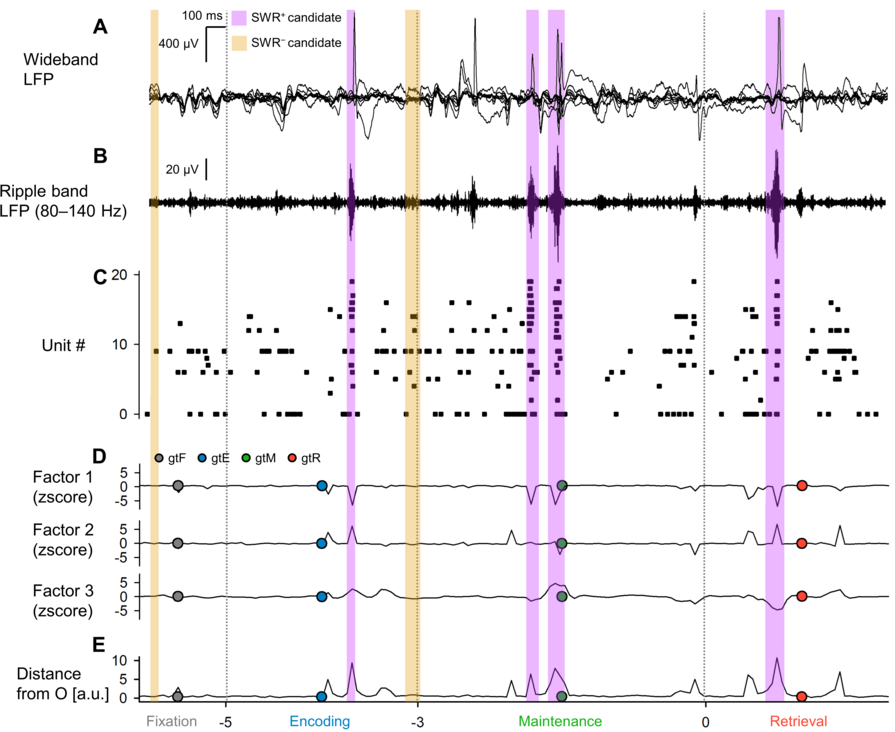
\includegraphics[width=1\textwidth]{./src/figures/.png/Figure_ID_01.png}
        	\caption{\textbf{Local Field Potential (LFP), Multiunit Activity, and Neural Trajectory of the Hippocampus during a Modified Sternberg Task} \cite{li_functional_2023, borders_hippocampal_2022, dimakopoulos_information_2022}}
\smallskip
\\
\textbf{\textit{A.}} Presented here are representative wideband LFP traces from iEEG signals, observed in the left hippocampal head during the execution of a modified Sternberg working memory task. The task involves fixation (1 s, \textit{gray}), encoding (2 s, \textit{blue}), maintenance (3 s, \textit{green}), and retrieval (2 s, \textit{red}) \cite{li_functional_2023, borders_hippocampal_2022, dimakopoulos_information_2022}. \textbf{\textit{B.}} Shown here are the corresponding ripple band LFP traces \cite{schomburg_spiking_2012, behrens_induction_2005, norimoto_hippocampal_2018}. \textbf{\textit{C.}} Illustrated here is the raster plot of multiunit spikes, produced from the LFP traces using a spike sorting algorithm \cite{niediek_reliable_2016}. \textbf{\textit{D.}} Indicated is the neural trajectory, established by the GPFA, based on the spike counts per unit within 50-ms bins \cite{yu_gaussian-process_2009}. The dotted circles depict the geometric median coordinates for each phase. \textbf{\textit{E.}} The distance of the trajectory from point $O$ is shown. It should be noted that the \textit{purple} and \textit{yellow} rectangles indicate the timings for SWR$^+$ candidates and SWR$^-$ candidates, which serve as controls for SWR$^+$, respectively \cite{van_vugt_hippocampal_2010, scoville_loss_1957, kay_hippocampal_2016, nader_memory_2003, wilson_reactivation_1994, nadasdy_replay_1999, lee_memory_2002}.
}
% width=1\textwidth
        	\label{fig:01}
        \end{figure*}
        \clearpage
        \begin{figure*}[ht]
            \pdfbookmark[2]{ID 02}{figure_id_02}
        	\centering
            \includegraphics[width=]{./src/figures/.png/Figure_ID_02.png}
        	\caption{\textbf{
State-dependent Hippocampal Neural Trajectory
}
\smallskip
\\
\textbf{\textit{A.}} This figure illustrates the neural trajectory in the first three dimensions, which are computed using the Gaussian Process Factor Analysis (GPFA). Each smaller dot represents the coordinates of a 50-ms neural trajectory bin, while larger dots marked in \textit{black} signify the geometric medians of successive phases in the Sternberg working memory task. These phases include fixation (\textit{gray}), encoding (\textit{blue}), maintenance (\textit{green}), and retrieval (\textit{red})\cite{yu_gaussian-process_2009}. \textbf{\textit{B.}} The graph displays the log-likelihood of GPFA models relative to the number of dimensions used for embedding multi-unit spikes in medial temporal lobe (MTL) regions. Importantly, the optimal value of dimensionality was identified as three, using the elbow method\cite{virtanen_scipy_2020}. \textbf{\textit{C.}} This section maps the distance between the neural trajectory and the origin ($O$) for the hippocampus (Hipp.), entorhinal cortex (EC), and amygdala (Amy.), and plots it against time from the commencement of the probe \cite{boran_dataset_2020}. \textbf{\textit{D.}} The following graph highlights the trajectory's distance from $O$ across MTL regions, with the hippocampus displaying the greatest distance, followed by the EC and Amygdala\cite{fernandez-ruiz_long-duration_2019}. \textbf{\textit{E.}} The final representation indicates the inter-phase trajectory distances within the MTL regions\cite{liu_consensus_2022}.
Abbreviations:
}
        	\label{fig:02}
        \end{figure*}
        \clearpage
        \begin{figure*}[ht]
            \pdfbookmark[2]{ID 03}{figure_id_03}
        	\centering
            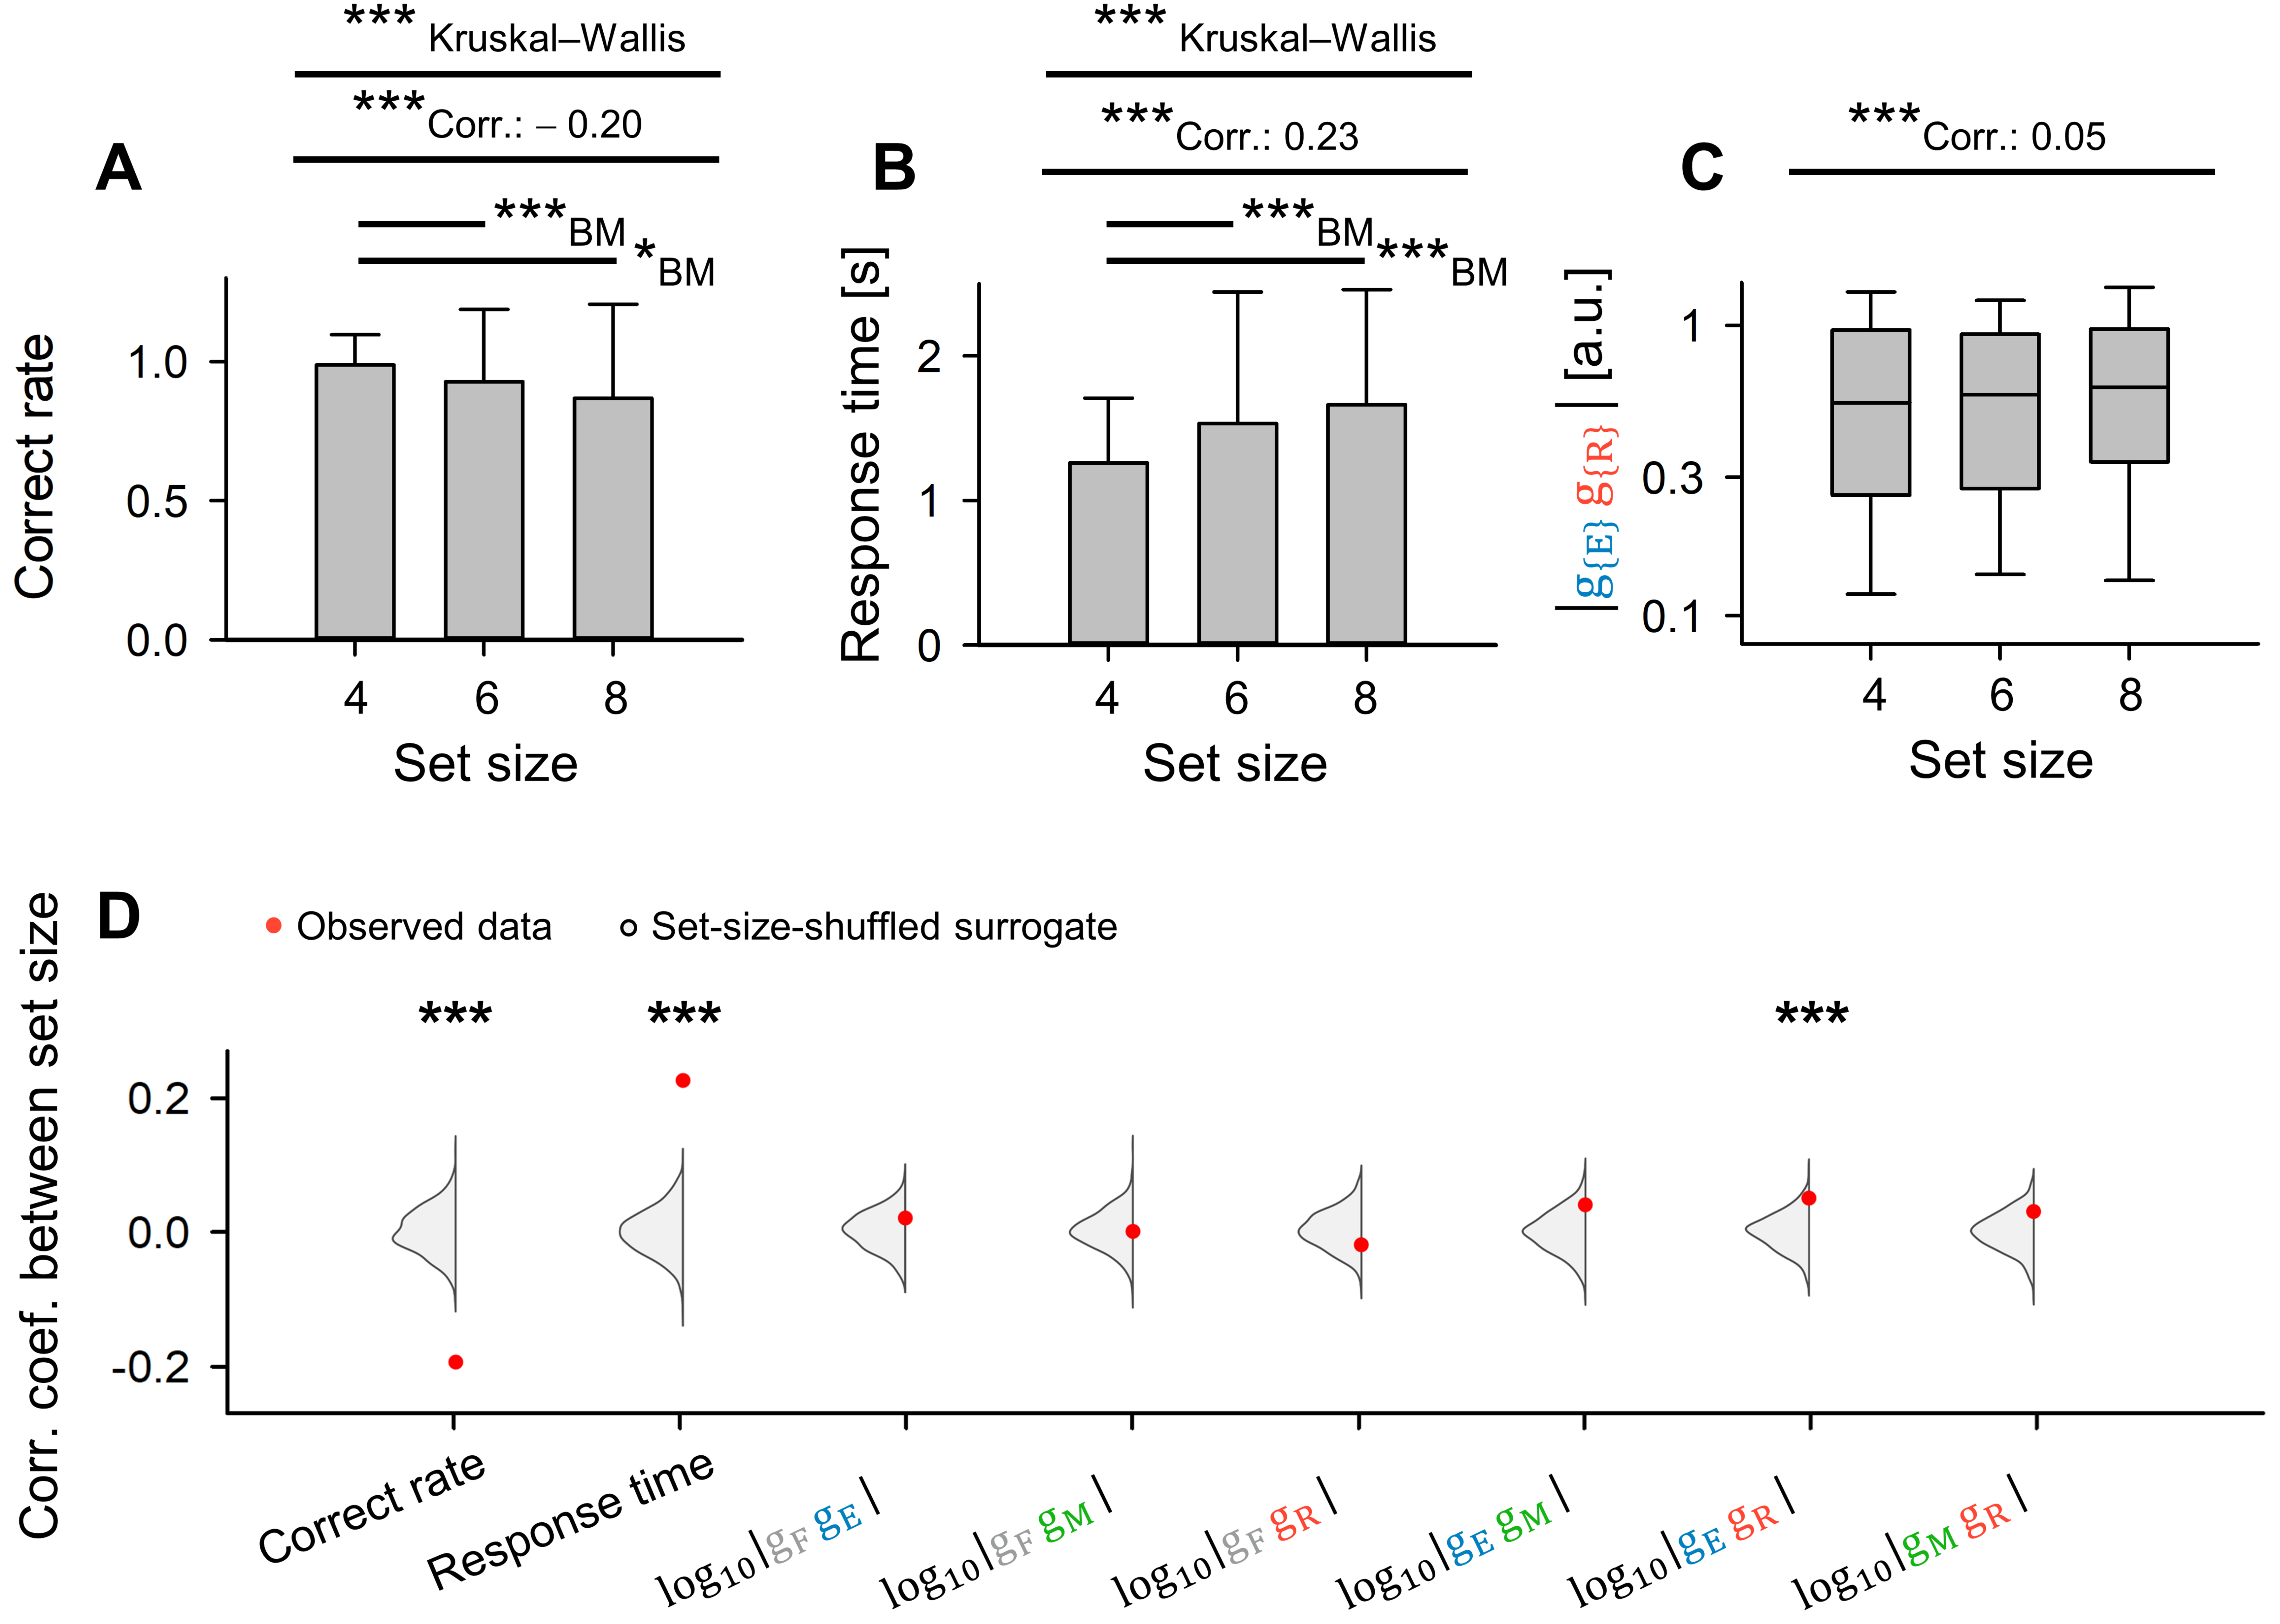
\includegraphics[width=1\textwidth]{./src/figures/.png/Figure_ID_03.png}
        	\caption{\textbf{
Dependence of Trajectory Distance on Memory Load Between Encoding and Retrieval States in the Hippocampus
}
\smallskip
\\
\textbf{\textit{A.}} A significant correlation has been noted between the set size (the number of letters to encode) and the correct rate in the WM task (coefficient = $-0.20$, ***\textit{p} $<$ 0.001) \cite{van_vugt_hippocampal_2010, li_functional_2023, borders_hippocampus_2022}. \textbf{\textit{B.}} There is a significant correlation between set size and response time (coefficient = $0.23$, ***\textit{p} $<$ 0.001) \cite{dimakopoulos_information_2022}.  \textbf{\textit{C.}} A correlation is also present between set size and the inter-phase distances between encoding and retrieval phases ($\Vert \mathrm{g_{E}g_{R}} \Vert$), albeit less significantly (correlation coefficient = 0.05) \cite{li_functional_2023}. \textbf{\textit{D.}} \textit{Red} dots represent the experimentally observed correlations between set size and the parameters listed: correct rate, response time, $\log_{10}{\Vert \mathrm{g_{F}g_{E}} \Vert}$, $\log_{10}{\Vert \mathrm{g_{F}g_{M}} \Vert}$, $\log_{10}{\Vert \mathrm{g_{F}g_{R}} \Vert}$, $\log_{10}{\Vert \mathrm{g_{E}g_{M}} \Vert}$, $\log_{10}{\Vert \mathrm{g_{E}g_{R}} \Vert}$, and $\log_{10}{\Vert \mathrm{g_{M}g_{R}} \Vert}$. The \textit{gray} kernel density plot depicts the corresponding set-size-shuffled surrogate measurements (\textit{n} = 1,000) (***\textit{p}s $<$ 0.001) \cite{norimoto_hippocampal_2018, hajos_input-output_2013}.
}
% width=1\textwidth
        	\label{fig:03}
        \end{figure*}
        \clearpage
        \begin{figure*}[ht]
            \pdfbookmark[2]{ID 04}{figure_id_04}
        	\centering
            \includegraphics[width=1\textwidth]{./src/figures/.png/Figure_ID_04.png}
        	\caption{\textbf{Detection of SWRs in Presumed CA1 Regions}
\smallskip
\\
\textbf{\textit{A.}} A two-dimensional Uniform Manifold Approximation and Projection (UMAP) projection of multi-unit spikes during potential SWRs (\textit{purple}) and non-SWRs (\textit{yellow}) periods is provided\cite{mcinnes_umap_2018}. \textbf{\textit{B.}} The cumulative density plot of silhouette scores, gauging the quality of UMAP clustering across the various hippocampal regions, is displayed (refer to Table~\ref{tab:02}). Areas that earned a silhouette score exceeding 0.60 (corresponding to the $75^{th}$ percentile), are marked as likely CA1 regions. The SWR and non-SWR periods within these potential CA1 regions were classified as SWRs and non-SWRs, correspondingly (\textit{n}s = 1,170)\cite{rousseeuw_silhouettes_1987}. \textbf{\textit{C.}} The distribution of durations for both SWRs (\textit{purple}) and non-SWRs (\textit{yellow}) are illustrated, following their respective definitions (93.0 [65.4] ms, median [IQR])\cite{girardeau_selective_2009}\cite{norman_hippocampal_2021}. \textbf{\textit{D.}} A depiction of the occurrence rate of SWRs (\textit{purple}) and non-SWRs (\textit{yellow}) over time since the start of stimulation, represented as a mean value \textpm 95\% confidence interval. It's important to acknowledge that due to closely spaced intervals, visual distinction can be challenging. Moreover, a noticeable rise in SWR occurrence was identified during the initial 400 ms of the retrieval phase (0.421 [Hz], *\textit{p} < 0.05, bootstrap test)\cite{buzsaki_hippocampal_2015}\cite{ego-stengel_disruption_2010}\cite{fernandez-ruiz_long-duration_2019}. \textbf{\textit{E.}} Distributions of ripple band peak amplitudes for non-SWRs (\textit{yellow}; 2.37 [0.33] times the standard deviation (SD) of the baseline, median [IQR]) and SWRs (\textit{purple}; 3.05 [0.85] times the SD of the baseline, median [IQR]) are shown. Substantial differences were found (***\textit{p} < 0.001, using the Brunner--Munzel test)\cite{norman_hippocampal_2019}\cite{diba_forward_2007}\cite{liu_consensus_2022}.
}
% width=1\textwidth
        	\label{fig:04}
        \end{figure*}
        \clearpage
        \begin{figure*}[ht]
            \pdfbookmark[2]{ID 05}{figure_id_05}
        	\centering
            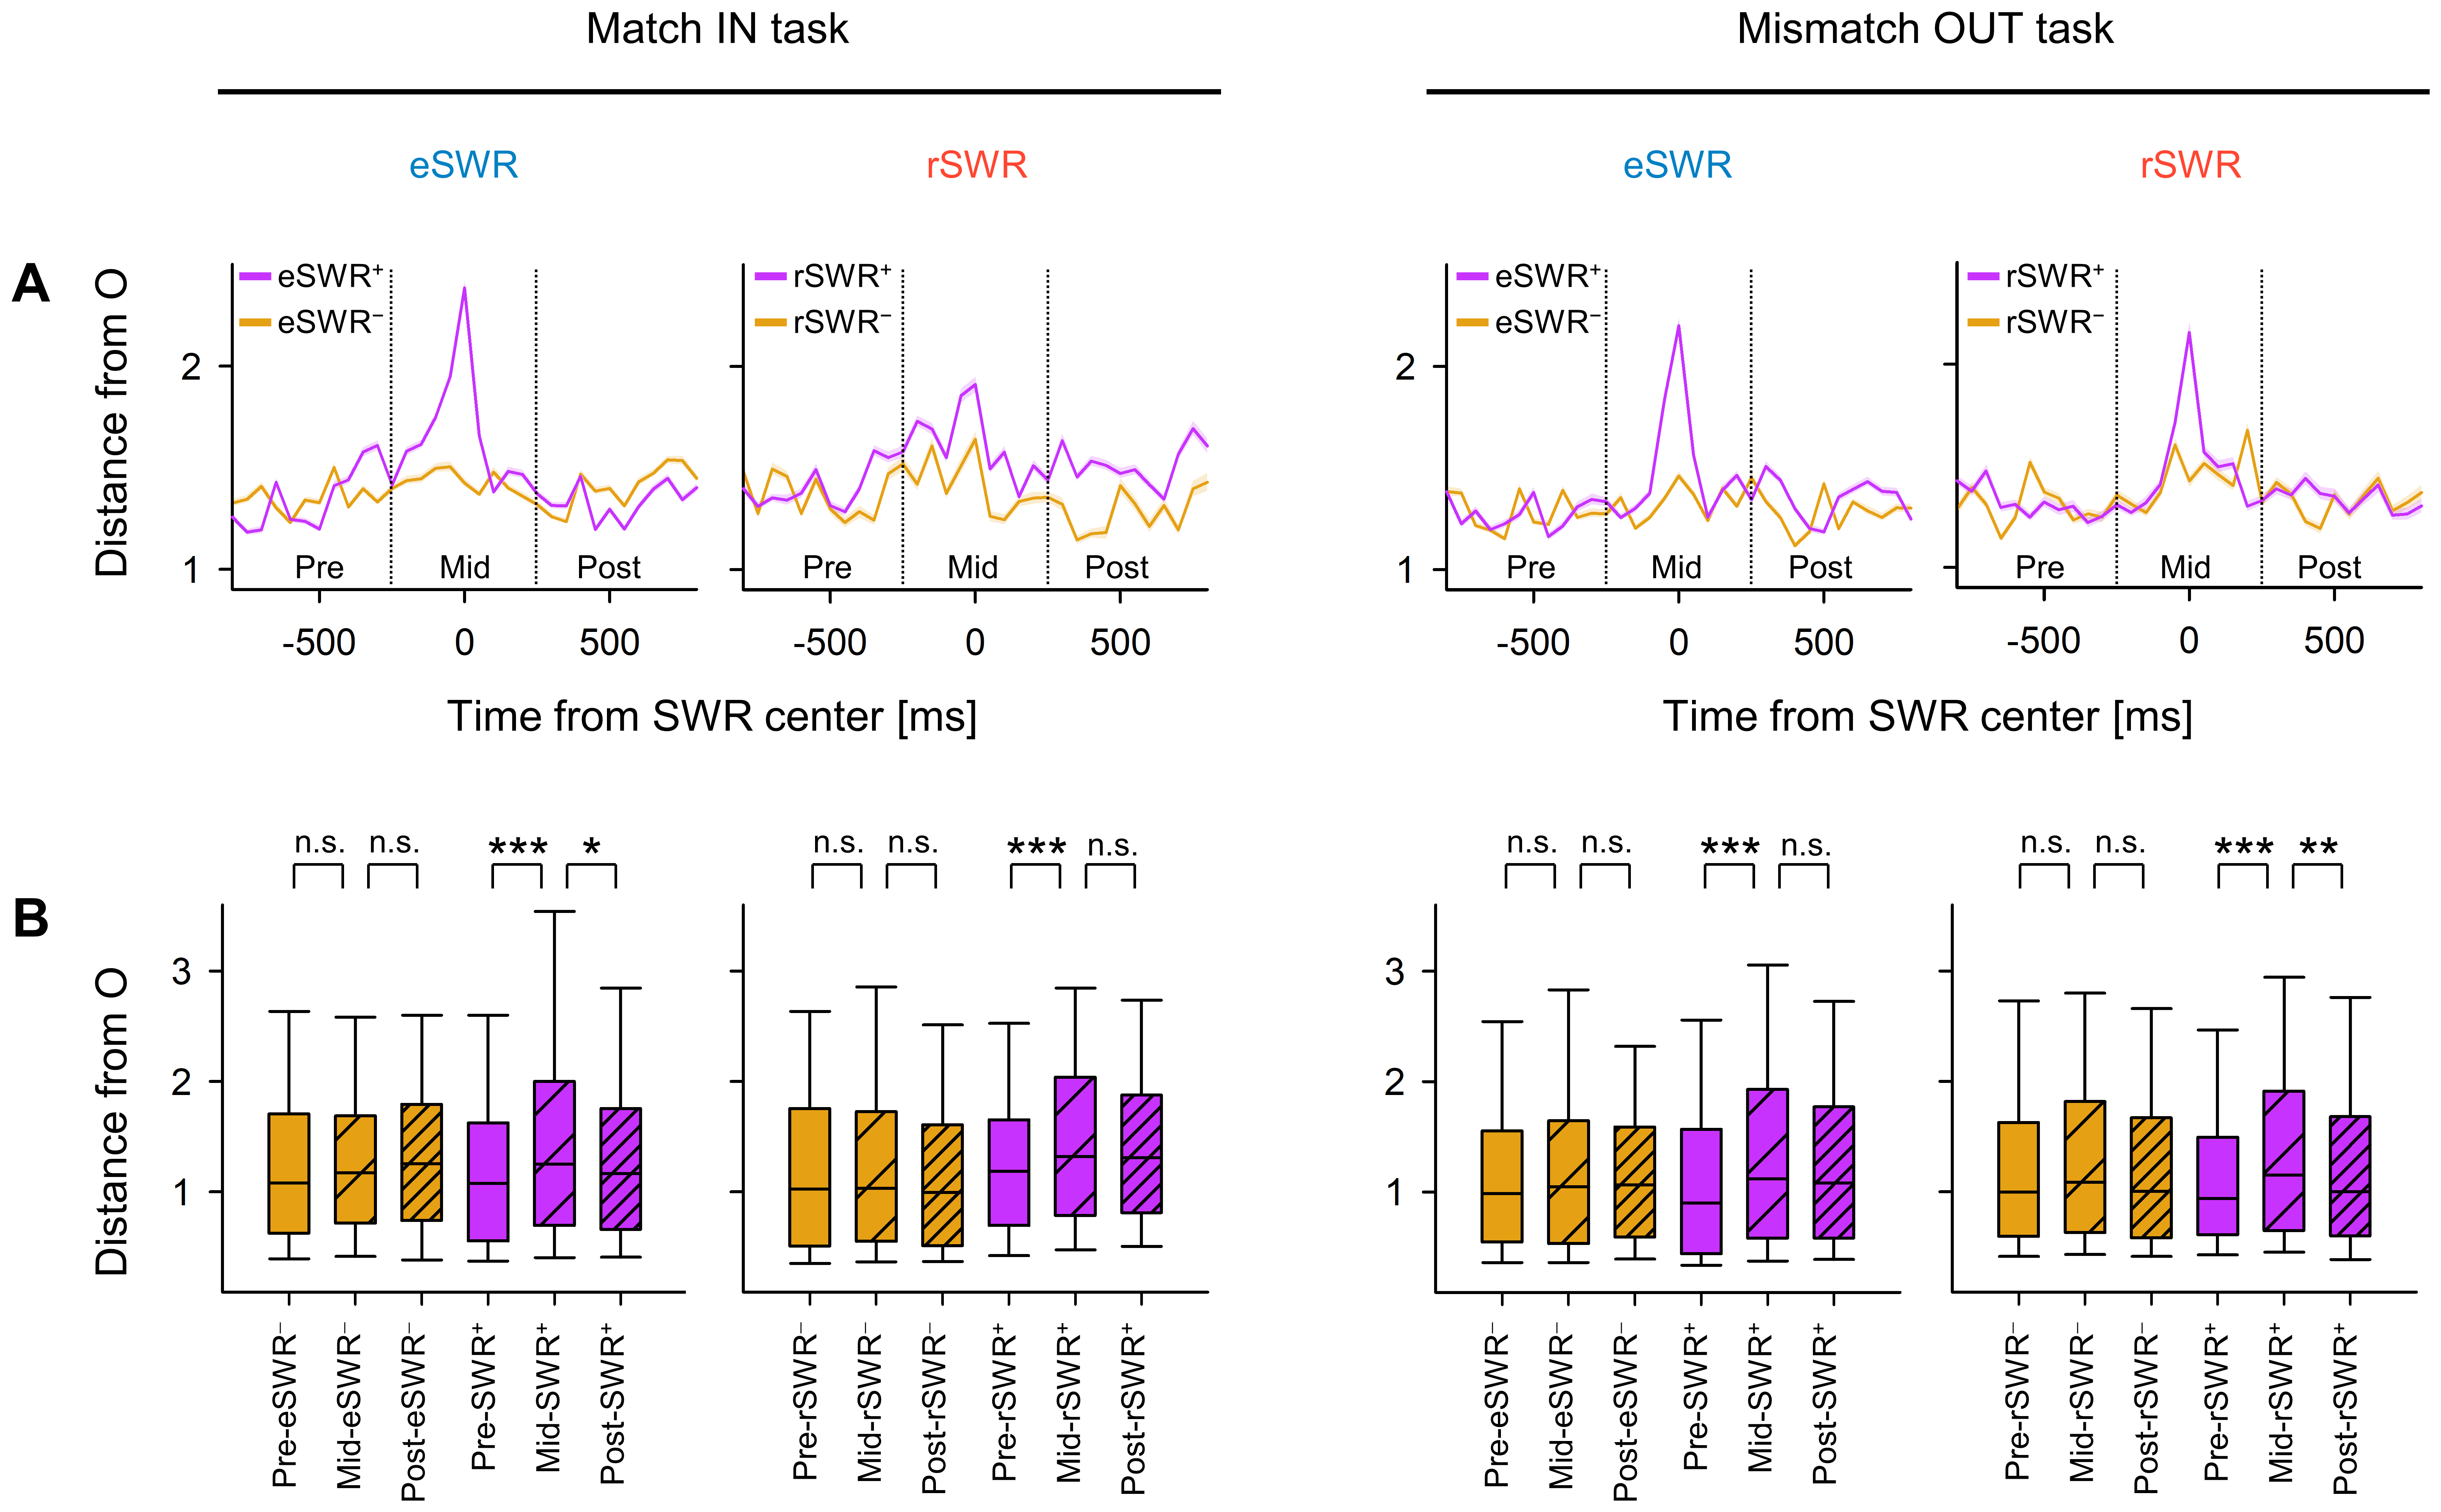
\includegraphics[width=1\textwidth]{./src/figures/.png/Figure_ID_05.png}
        	\caption{\textbf{Transient Changes in Neural Trajectory During SWR}
\smallskip
\\
\textbf{\textit{A.}} Represents the mean distance from the origin ($O$) of the peri-sharp-wave-ripple (SWR) trajectory, paired with a 95\% confidence interval that might not be visible due to its limited range \cite{girardeau_selective_2009,norman_hippocampal_2019,buzsaki_hippocampal_2015}. \textbf{\textit{B.}} Illustrates the distance from the origin ($O$) during the intervals pre-, mid-, and post-SWR (*\textit{p} $<$ 0.05, **\textit{p} $<$ 0.01, ***\textit{p} $<$ 0.001; according to the Brunner--Munzel test \cite{boran_persistent_2019}). Defined terms include: SWR, sharp-wave ripple events; eSWR, SWR that occur during the encoding phase; rSWR, SWR happening in the retrieval phase; SWR$^+$, a SWR event; SWR$^-$, the control events matched with SWR$^+$; pre-, mid-, or post-SWR, the time segments from $-800$ to $-250$ ms, from $-250$ to $+250$ ms, and from $+250$ to $+800$ ms, respectively, all in relation to the SWR center.
}
% width=1\textwidth
        	\label{fig:05}
        \end{figure*}
        \clearpage
        \begin{figure*}[ht]
            \pdfbookmark[2]{ID 06}{figure_id_06}
        	\centering
            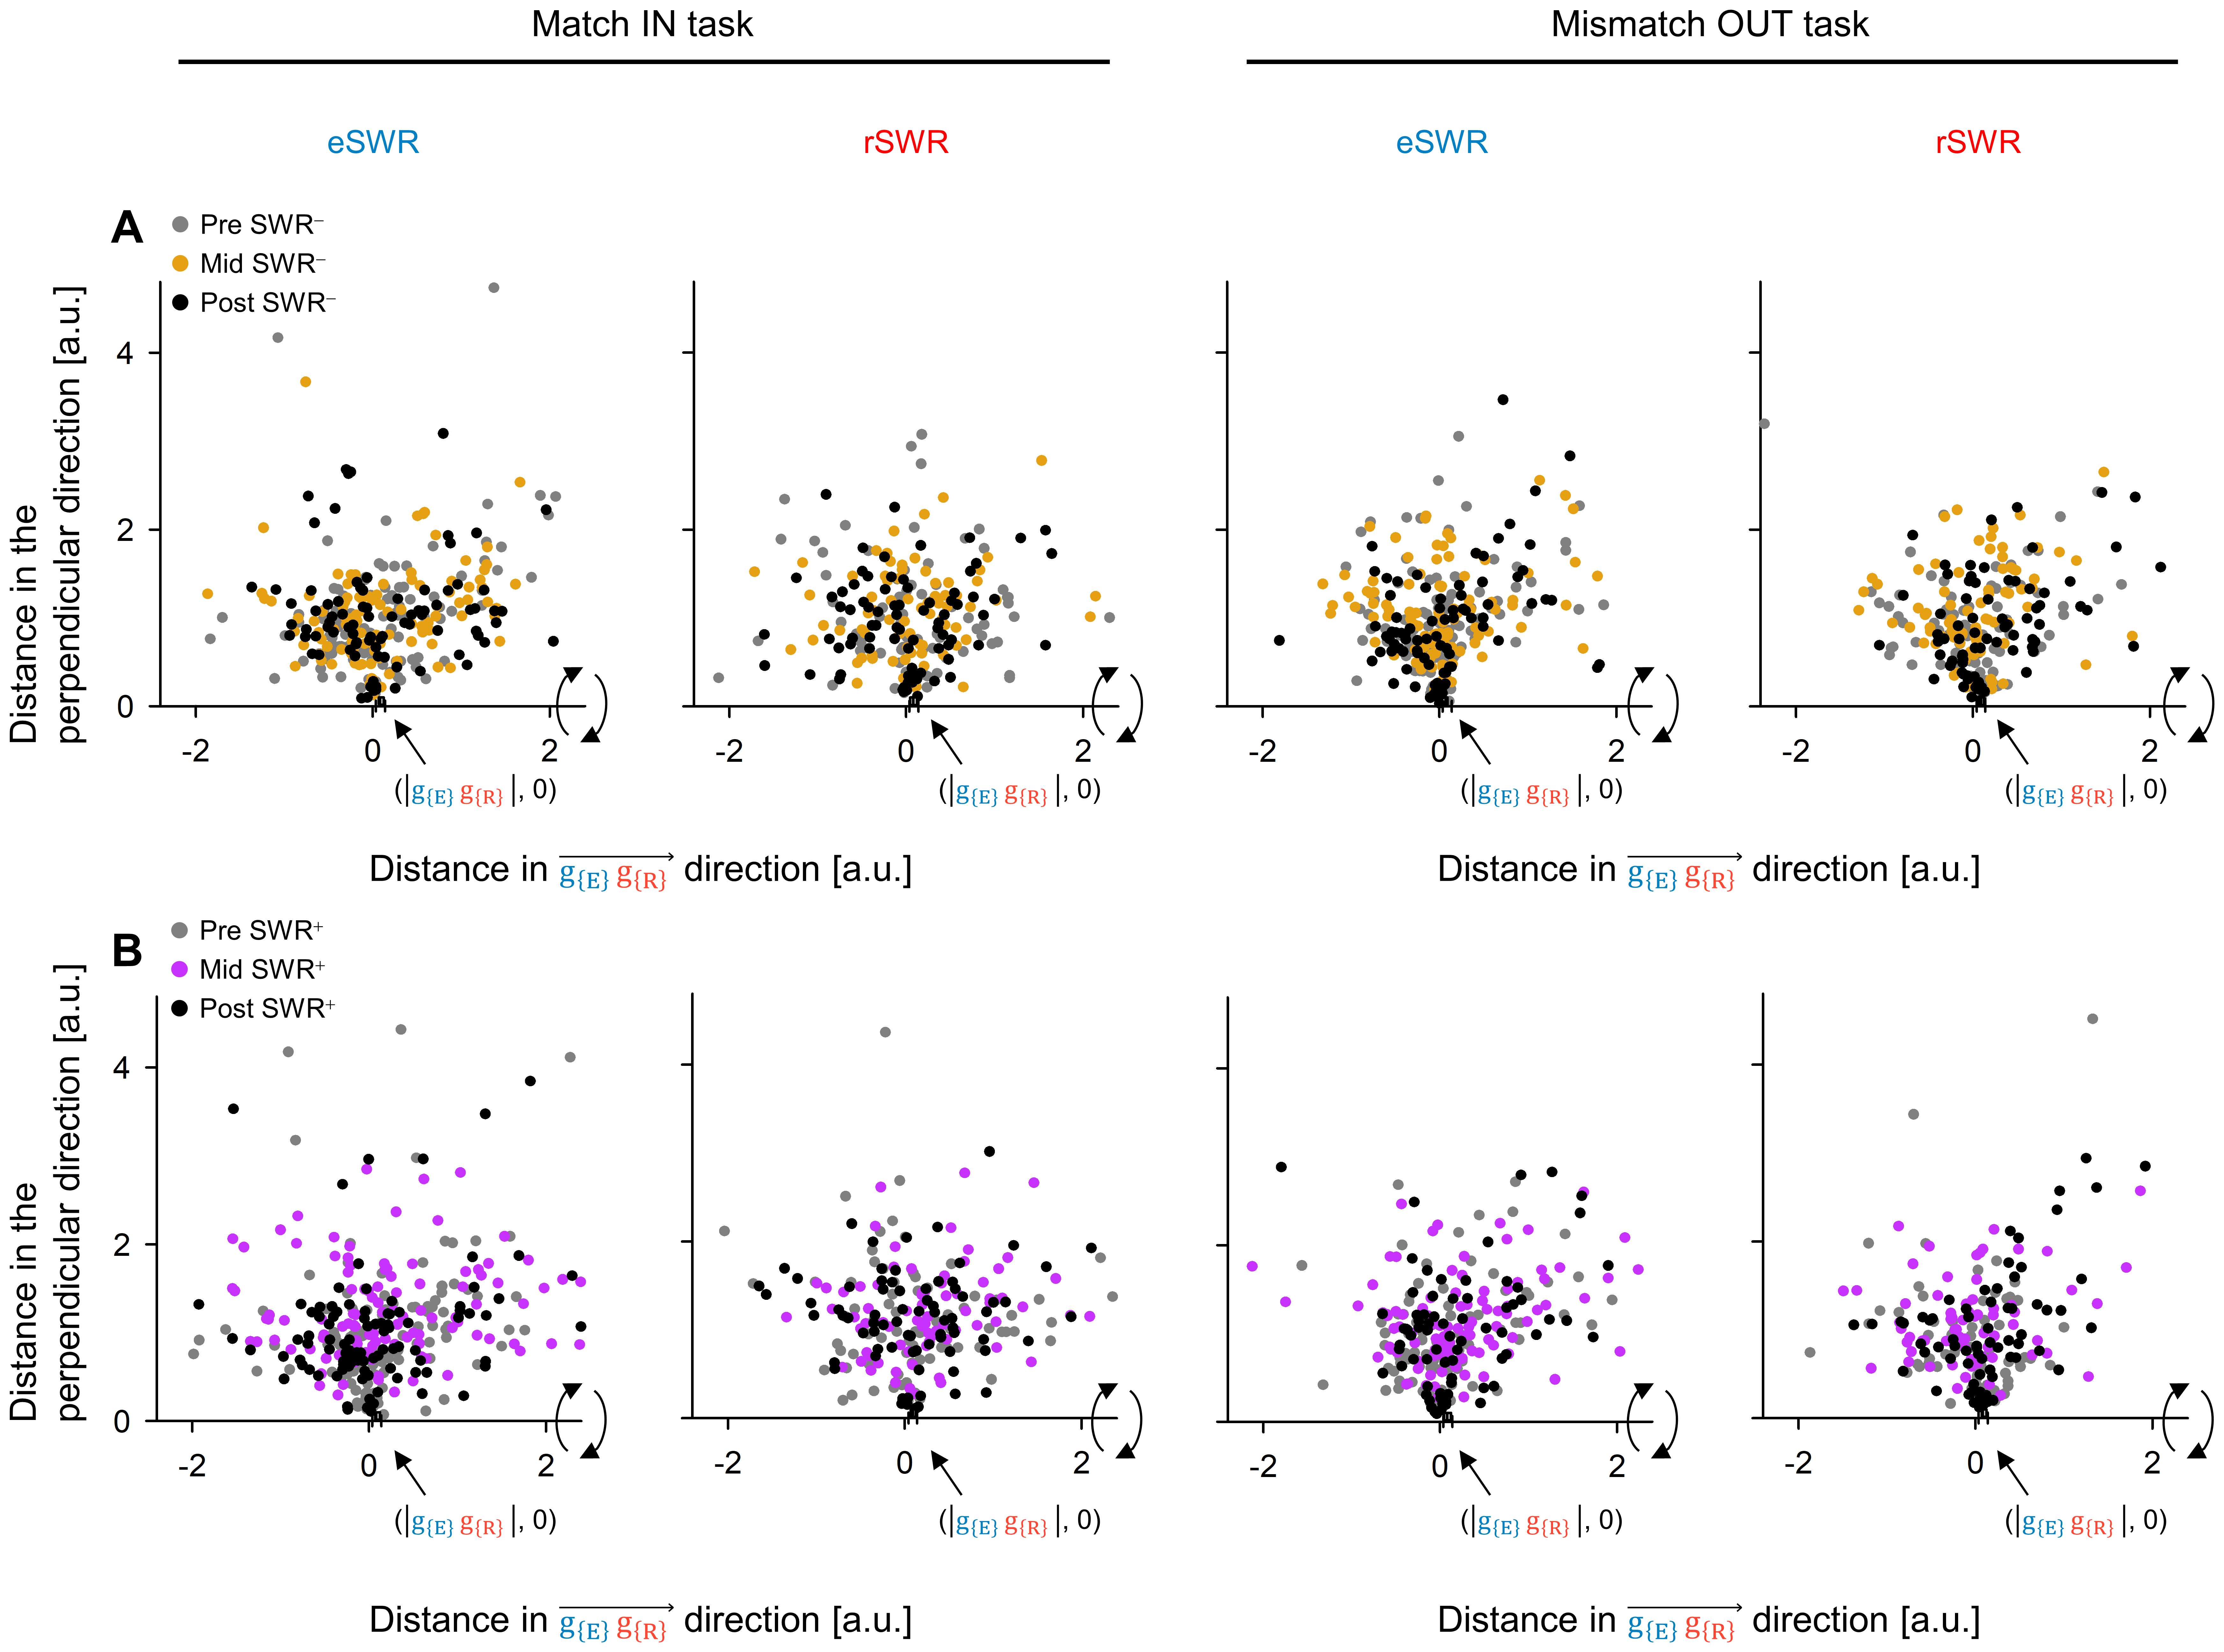
\includegraphics[width=1\textwidth]{./src/figures/.png/Figure_ID_06.png}
        	\caption{\textbf{Visualizing Neural Trajectories During Sharp-Wave Ripple Events in a Two-Dimensional Space}

\smallskip

\\
This illustration showcases neural trajectories association with hippocampal activity during Sharp-Wave Ripple (SWR) events, as displayed in a two-dimensional context. \textbf{\textit{A.}} It presents exemplar trajectories of the pre- (\textit{gray}), mid- (\textit{yellow}), and post-SWR$^-$ (\textit{black}) phases of an SWR event~\cite{buzsaki_hippocampal_2015}. \textbf{\textit{B.}} Shown here are the trajectories that align with SWR$^+$ circumstances, as observed against the SWR$^-$ backgrounds~\cite{fernandez-ruiz_long-duration_2019}. The magnitude of $\lVert \mathrm{g_{E}g_{R}} \rVert$ displays patterns of variation across sessions~\cite{liu_consensus_2022}. The projection protocol can be described as follows: initially, $\mathrm{g_{E}}$ was positioned at the origin $O$ (0,0), and $\mathrm{g_{R}}$ at ($\lVert \mathrm{g_{E}g_{R}} \rVert$, 0), achieved through linear transformation~\cite{kim_corticalhippocampal_2022}. Later, a rotation of the point cloud around the $\mathrm{g_{E}g_{R}}$ axis (the x-axis) was performed, allowing compatibility with a two-dimensional space~\cite{yu_gaussian-process_2009}. Consequently, both the distances from $O$ and the angles relative to the $\mathrm{g_{E}g_{R}}$ axis maintained the same attributes as in their three-dimensional arrangement~\cite{mcinnes_umap_2018}. Acronyms and terms used: SWR refers to Sharp-Wave Ripple events; eSWR stands for SWR during the encoding phase; rSWR indicates SWR during the retrieval phase; SWR$^+$ represents an SWR event; SWR$^-$ designates the control event for SWR$^+$; the terms pre-SWR, mid-SWR, and post-SWR delineate the time intervals ranging from $-800$ to $-250$ ms, from $-250$ to $+250$ ms, and from $+250$ to $+800$ ms from the center of an SWR event, respectively~\cite{zhang_hippocampal_2022}.
}
% width=1\textwidth
        	\label{fig:06}
        \end{figure*}
        \clearpage
        \begin{figure*}[ht]
            \pdfbookmark[2]{ID 07}{figure_id_07}
        	\centering
            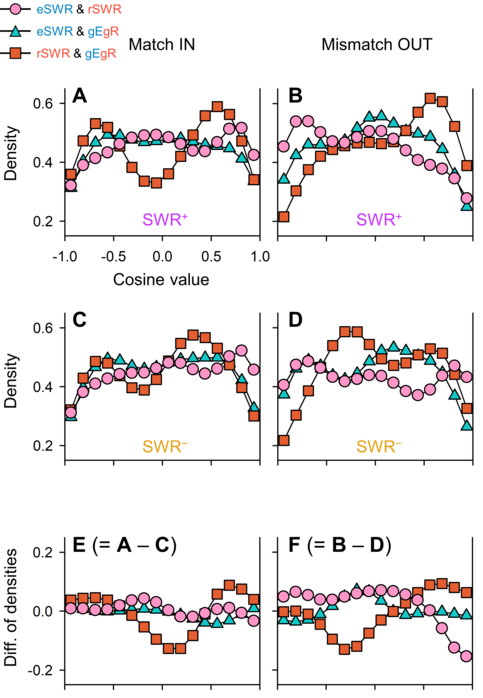
\includegraphics[width=0.5\textwidth]{./src/figures/.png/Figure_ID_07.png}
        	\caption{\textbf{
Directionality of Neural Trajectories in SWR Based on Encoding and Retrieval States
}
\smallskip
\\
\textbf{\textit{A--B}} The Kernel Density Estimation (KDE) distributions of $\protect\overrightarrow{{\mathrm{eSWR^+}}} \cdot \protect\overrightarrow{{\mathrm{rSWR^+}}}$ (\textit{pink circles}), $\protect\overrightarrow{{\mathrm{eSWR^+}}} \cdot \protect\overrightarrow{{\mathrm{g_{E}g_{R}}}}$ (\textit{blue triangles}), and $\protect\overrightarrow{{\mathrm{rSWR^+}}} \cdot \protect\overrightarrow{{\mathrm{g_{E}g_{R}}}}$ (\textit{red rectangles}) in the Match IN (\textit{A}) and Mismatch OUT tasks (\textit{B}) are shown~\cite{li_functional_2023}. \textbf{\textit{C--D}} The analogous distributions for these tasks when $\mathrm{SWR^-}$ replaces $\mathrm{SWR^+}$ are presented~\cite{dimakopoulos_information_2022}. \textbf{\textit{E--F}} The contrasts between the distributions of $\mathrm{SWR^+}$ and $\mathrm{SWR^-}$ underscore the SWR components (\textit{E} = \textit{C} $-$ \textit{A}; \textit{F} = \textit{B} $-$ \textit{D}), where the biphasic distributions of $\protect\overrightarrow{{\mathrm{rSWR^-}}} \cdot \protect\overrightarrow{{\mathrm{g_{E}g_{R}}}}$ highlight the neural oscillations between encoding and retrieval states during the Sternberg task~\cite{borders_hippocampus_2022}. Conversely, the Mismatch OUT task revealed an inverse relationship between $\protect\overrightarrow{{\mathrm{eSWR^+}}}$ and $\protect\overrightarrow{{\mathrm{rSWR^+}}}$ (\textit{pink circles}), a phenomenon not noted in the Match IN task (\textbf{\textit{E--F}})~\cite{naber_reciprocal_2001,van_strien_anatomy_2009}. Lastly, observed transitions from retrieval to encoding for the SWR components were evident in both the Match IN and Mismatch OUT tasks (\textit{red rectangles} in \textit{E--F})~\cite{niediek_reliable_2016,schomburg_spiking_2012}.
}
% width=0.5\textwidth
        	\label{fig:07}
        \end{figure*}


%%%%%%%%%%%%%%%%%%%%%%%%%%%%%%%%%%%%%%%%%%%%%%%%%%%%%%%%%%%%%%%%%%%%%%%%%%%%%%%%
%% END
%%%%%%%%%%%%%%%%%%%%%%%%%%%%%%%%%%%%%%%%%%%%%%%%%%%%%%%%%%%%%%%%%%%%%%%%%%%%%%%%

\end{document}
